\documentclass[12pt, letterpaper]{article}

% --- PAQUETES DE IDIOMA Y FORMATO ---
\usepackage[utf8]{inputenc}
\usepackage[spanish]{babel}
\usepackage[margin=2.5cm]{geometry}
\usepackage{graphicx} 
\usepackage{hyperref} 
\usepackage{xcolor}   
\usepackage{listings}
\usepackage{booktabs} 
\usepackage{float}

% --- CONFIGURACIÓN PARA EL CÓDIGO JAVA ---
\definecolor{codegreen}{rgb}{0,0.6,0}
\definecolor{codegray}{rgb}{0.5,0.5,0.5}
\definecolor{codepurple}{rgb}{0.58,0,0.82}
\definecolor{backcolour}{rgb}{0.95,0.95,0.92}

\lstdefinestyle{mystyle}{
	backgroundcolor=\color{backcolour},   
	commentstyle=\color{codegreen},
	keywordstyle=\color{magenta},
	numberstyle=\tiny\color{codegray},
	stringstyle=\color{codepurple},
	basicstyle=\ttfamily\footnotesize,
	breakatwhitespace=false,         
	breaklines=true,                 
	captionpos=b,                    
	keepspaces=true,                 
	numbers=left,                    
	numbersep=5pt,                  
	showspaces=false,                
	showstringspaces=false,
	showtabs=false,                  
	tabsize=2
}
\lstset{style=mystyle}

% --- INICIO DEL DOCUMENTO ---
\begin{document}
	
	% --- PORTADA ---
	\begin{titlepage}
		\centering
		\vspace*{0.5cm}
		
		
\includegraphics[width=2.8cm]{logo_unam.png} 
		\hfill
		
\includegraphics[width=2.8cm]{logo_fi.png} 
		\\[1.5cm]
		
		{\Huge \textbf{Universidad Nacional Autónoma de México}}\\[0.5cm]
		{\LARGE \textbf{Facultad de Ingeniería}}\\[1.5cm]
		
		{\Large Asignatura: Programación Orientada a Objetos}\\[0.5cm]
		{\Large Proyecto: Sistema Bancario en Java}\\[1.5cm]
		
		% Título del Reporte
		\rule{\linewidth}{0.5mm} \\[0.4cm]
		{ \huge \bfseries Reporte Técnico Final: \\ Implementación de Sistema Bancario (Core Banking) }\\[0.4cm]
		\rule{\linewidth}{0.5mm} \\[2.5cm]
		
		\begin{flushleft}
			\Large \textbf{Equipo de Desarrollo:}\\
			\vspace{0.3cm}
			\normalsize
			$\bullet$ Francisco José Coutiño Morales (Núm. Cta: 425121623)\\ 
			$\bullet$ Ernesto Flamenco Villaseñor (Núm. Cta: 319170599)\\
			$\bullet$ Jaime Erick Torres Nava (Núm. Cta: 322289976)\\
		\end{flushleft}
		
		\vfill
		{\large \today}\\[1cm]
	\end{titlepage}
	
	% --- ÍNDICE ---
	\newpage
	\tableofcontents
	\newpage
	
	% =========================================================================
	% --- SECCIÓN 1: INTRODUCCIÓN ---
	% =========================================================================
	\section{Introducción}
	El presente documento detalla la arquitectura, las decisiones de diseño y el flujo de desarrollo del proyecto ``Sistema Bancario El Bienestar''. El sistema fue desarrollado en el lenguaje Java, aplicando rigorosamente los paradigmas de la Programación Orientada a Objetos (POO) y haciendo uso intensivo del \textit{Java Collections Framework} para el manejo eficiente de la información en memoria.
	
	El objetivo principal de esta fase final fue modelar las entidades básicas del dominio bancario, construir un núcleo transaccional capaz de gestionar clientes, cuentas de débito, pagarés de inversión y tarjetas de crédito, y garantizar la integridad de los fondos simulando operaciones reales del sistema financiero.
	
	% =========================================================================
	% --- SECCIÓN 2: MARCO TEÓRICO ---
	% =========================================================================
	\section{Marco Teórico: Jerarquía de Colecciones en Java}
	
	El Java Collections Framework es una arquitectura para almacenar y manipular grupos de objetos de forma eficiente. Estas estructuras están optimizadas a nivel de memoria y algoritmos de búsqueda. La jerarquía se divide principalmente en dos ramas: 
	\begin{itemize}
		\item \textbf{Interfaz Collection:} De ella heredan las interfaces List y Set.
		\item \textbf{Interfaz Map:} Maneja pares clave-valor.
	\end{itemize}
	
	\subsection{Análisis de Complejidad por Interfaz}
	
	\subsubsection{Listas (List)}
	Permiten elementos duplicados y mantienen el orden de inserción. Un \texttt{ArrayList} utiliza un arreglo dinámico que se redimensiona automáticamente, permitiendo acceso en $\mathcal{O}(1)$. Por otro lado, \texttt{LinkedList} utiliza nodos doblemente enlazados, optimizando las inserciones en los extremos.
	
	\subsubsection{Conjuntos (Set)}
	Prohíben la existencia de elementos duplicados. Un \texttt{HashSet} está respaldado por una tabla hash, ofreciendo operaciones matemáticas de conjuntos con un rendimiento promedio de inserción y búsqueda de $\mathcal{O}(1)$.
	
	\subsubsection{Tablas Hash (Map)}
	Almacenan información mediante una relación de ``Clave-Valor'', donde cada clave debe ser única. Mapean las llaves a ``cubetas'' (\textit{buckets}) en memoria, permitiendo búsquedas virtualmente instantáneas de complejidad $\mathcal{O}(1)$.
	
	\begin{table}[h]
		\centering
		\begin{tabular}{@{}llll@{}}
			\toprule
			\textbf{Estructura} & \textbf{¿Permite Duplicados?} & \textbf{¿Mantiene Orden?} & \textbf{Acceso a Datos} \\ \midrule
			List & Sí & Sí (por inserción) & Por índice (0, 1, 2...) \\
			Set & No & No (generalmente) & Por iteración o búsqueda \\
			Map & Solo en los valores & No & Por clave única \\ \bottomrule
		\end{tabular}
		\caption{Diferencias operativas entre List, Set y Map.}
	\end{table}
	
	% =========================================================================
	% --- SECCIÓN 3: ARQUITECTURA Y JUSTIFICACIÓN ---
	% =========================================================================
	\section{Arquitectura del Modelo de Datos}
	
	\subsection{Justificación Arquitectural: Desacoplamiento de Entidades}
	Una de las decisiones de diseño más importantes frente a implementaciones triviales fue la \textbf{separación estricta entre el ID del Cliente y el Número de Cuenta}. 
	
	En el dominio bancario real, un cliente posee múltiples productos. Al separar los identificadores, la entidad \texttt{Cliente} funciona como un expediente que encapsula colecciones de diversas cuentas (Cardinalidad 1:N), permitiendo que el sistema escale. Además, por seguridad, el Número de Cuenta es público (para recibir transferencias), mientras que el ID de Cliente es información sensible.
	
	\subsection{Evolución de Tipos de Dato (De la V1 a la Final)}
	Durante la planificación (V1), el número de cuenta y el ID se introducían como \texttt{String}. En esta versión final se ejecutó la refactorización a tipos primitivos enteros (\texttt{int}):
	\begin{itemize}
		\item \textbf{Restricción Numérica:} Garantiza de manera nativa que el sistema rechace caracteres alfabéticos, evitando excepciones de formato.
		\item \textbf{Eficiencia:} Optimiza el procesamiento numérico y el cálculo de colisiones (\textit{hashing}) dentro del \texttt{HashMap} y los \texttt{HashSet}.
	\end{itemize}
	Para lograr esto, se implementó la clase \texttt{java.util.Random} en el \texttt{GestorBanco}, la cual asigna automáticamente IDs de 9 dígitos únicos al registrar clientes.
	
	% =========================================================================
	% --- SECCIÓN 4: IMPLEMENTACIÓN PRÁCTICA DE COLECCIONES ---
	% =========================================================================
	\section{Implementación de Estructuras en el Código}
	Para optimizar el rendimiento y cumplir con las reglas de negocio, se asignó una estructura específica a cada necesidad operativa:
	
	\subsection{Uso de Map (Directorio Global)}
	En la clase \texttt{GestorBanco}, se implementó un \texttt{Map<Integer, Cliente>}. La llave es el número de cliente (\texttt{int}) y el valor es el objeto \texttt{Cliente}. Esto permite encontrar cualquier perfil de manera instantánea $\mathcal{O}(1)$ al teclear su ID en el cajero.
	
	\subsection{Uso de Set (Cartera de Productos Únicos)}
	Se utilizaron tres colecciones \texttt{HashSet} dentro de la clase \texttt{Cliente} para separar lógicamente su \texttt{CuentaBasica}, \texttt{CuentaInversion} y \texttt{TarjetaCredito}. Esto asegura matemáticamente que un cliente no pueda tener dos contratos con el mismo número de folio clonado.
	
	\subsection{Uso de LinkedList (Historial Transaccional LIFO)}
	A diferencia de la V1 (donde se propuso \texttt{ArrayList}), el historial de la clase \texttt{Movimiento} se refactorizó a \texttt{LinkedList<Movimiento>}. Un estado de cuenta requiere mostrar la transacción más reciente arriba. Esto dicta un comportamiento \textbf{LIFO} (Last-In, First-Out). Usando el método \texttt{addFirst()}, la inserción ocurre en $\mathcal{O}(1)$, desplazando los nodos anteriores más rápido que redimensionando un arreglo estático.
	
	% =========================================================================
	% --- SECCIÓN 5: ANÁLISIS TÉCNICO Y CORRECCIONES ---
	% =========================================================================
	\section{Flujo de Trabajo y Lógica de Negocio Transaccional}
	El desarrollo siguió un enfoque iterativo. Tras programar el menú interactivo con la clase \texttt{Scanner}, se detectaron y corrigieron vulnerabilidades críticas en la simulación financiera:
	
	\subsection{Prevención de ``Dinero Fantasma''}
	Durante las pruebas de caja blanca, se observó que el sistema permitía abrir contratos de inversión y pagar deudas de tarjetas de crédito sin afectar el saldo del cliente (creando capital de la nada). 
	
	Para solucionarlo simulando un banco real, se modificó el flujo del método en \texttt{GestorBanco}. Ahora, el sistema exige el número de la \texttt{CuentaBasica} origen, ejecuta el método booleano \texttt{retirar(monto)}, y \textbf{solo si este retorna true} (confirmando liquidez), procede a instanciar el contrato de inversión o a invocar el método \texttt{abonarDeuda()} de la tarjeta.
	
	\subsection{Explicación de Bloques de Código Clave}
	A continuación, se detalla la lógica detrás de instrucciones fundamentales:
	
	\begin{itemize}
		\item \textbf{\texttt{sn.nextLine();}:} Usado tras leer variables con \texttt{nextInt()} o \texttt{nextDouble()}. Java deja el carácter de salto de línea (\textbackslash n) en el flujo. Limpiar el \textit{buffer} evita que el menú del cajero se rompa al leer el siguiente \texttt{String}.
		\item \textbf{\texttt{return !cuentas.isEmpty();}:} Una validación booleana elegante. El banco exige poseer una cuenta básica para poder invertir. En lugar de un \texttt{if} largo, se niega el estado del \texttt{HashSet}; si no está vacío, devuelve \texttt{true}, autorizando la transacción.
		\item \textbf{\texttt{inversiones.remove(inversionTerminada);}:} Al liquidar una inversión, esta instrucción busca la referencia exacta del objeto en memoria dentro del \texttt{Set} y lo destruye, cerrando el contrato sin dejar \textit{memory leaks}.
	\end{itemize}
	
	% =========================================================================
	% --- SECCIÓN 6: UML Y CONCLUSIÓN ---
	% =========================================================================
	\section{Análisis de Diagrama UML y Trazabilidad}
	A continuación, se presenta el modelo conceptual diseñado para el proyecto:
	
	\begin{figure}[H]
		\centering
		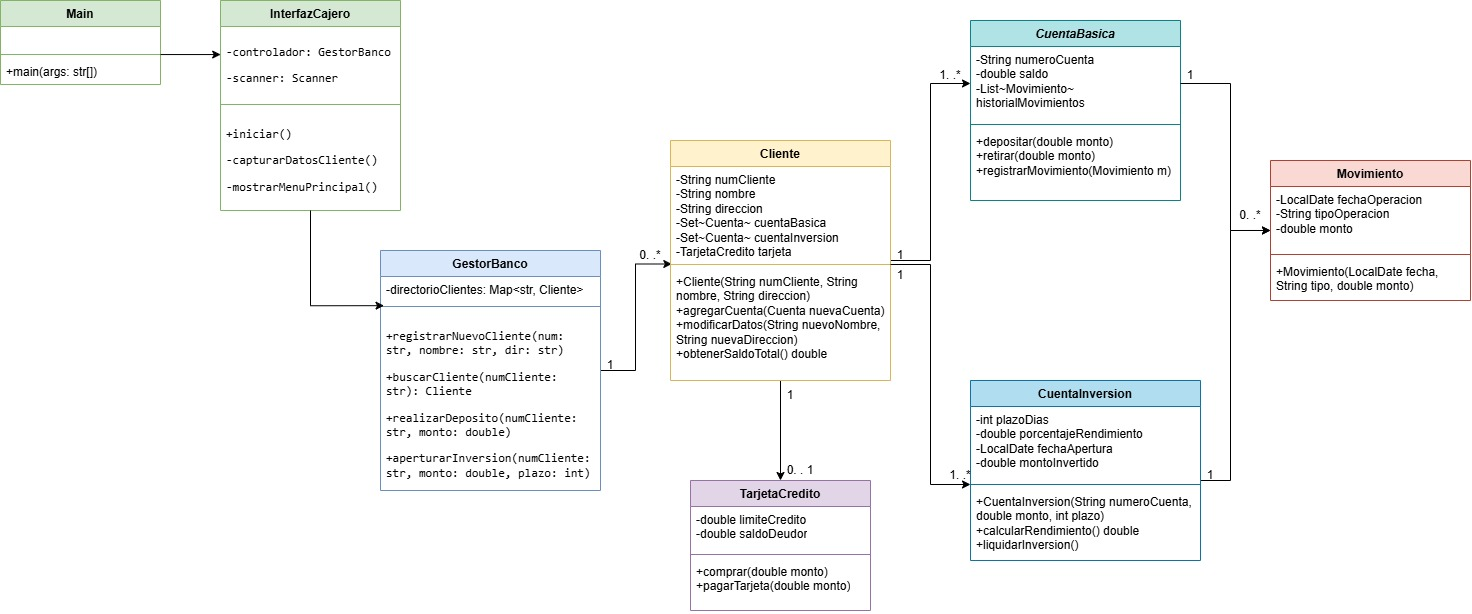
\includegraphics[width=0.9\textwidth]{Diagrama_UML_SistemaBancario.jpg} 
		\caption{Diagrama UML inicial del Sistema Bancario}
		\label{fig:uml}
	\end{figure}
	
	\subsection{Cumplimiento y Desviaciones del Modelo Original}
	El sistema final cumple con la arquitectura de la Figura \ref{fig:uml}, con ligeros ajustes de modernización:
	\begin{enumerate}
		\item \textbf{Fusión de Interfaz:} La propuesta \texttt{InterfazCajero} fue absorbida por el método \texttt{main} de \texttt{SistemaBancario} para centralizar el \texttt{Scanner} y mantener bajo acoplamiento.
		\item \textbf{Fechas Precisas:} En lugar de \texttt{LocalDate} para la clase \texttt{Movimiento}, el uso nativo de \textit{timestamps} garantiza precisión milimétrica en auditorías, dándole un enfoque realista.
	\end{enumerate}
	
	\section{Conclusiones}
	La evolución desde la Versión 1 hasta esta entrega final demuestra cómo la correcta aplicación teórica del \textit{Collections Framework} resuelve problemas de rendimiento en el mundo real. Se logró construir un núcleo transaccional robusto que no solo registra datos, sino que simula de manera precisa la estricta lógica financiera (como el fondeo condicionado) de una institución bancaria verdadera.
	
\end{document}